\documentclass[11pt]{article}
\usepackage{enumerate, comment}
\usepackage{hyperref}
\usepackage{amsmath,amssymb,amsthm}
\usepackage{ wasysym }
\usepackage{ marvosym }
\usepackage{ textcomp }
\usepackage{xcolor}
\usepackage{graphicx}
\usepackage{epstopdf}
\usepackage{wrapfig}
\usepackage{epigraph}
%\usepackage[bottom=1.5in]{geometry}

\newcommand{\N}{\mathbb{N}}
\newcommand{\Z}{\mathbb{Z}}
\newcommand{\Q}{\mathbb{Q}}
\newcommand{\R}{\mathbb{R}}
\newcommand{\C}{\mathbb{C}}
\newcommand{\Aut}[1]{\ensuremath{ \aaut \left (#1 \right ) }}
\newcommand{\ins}[1]{\ensuremath{{#1}^{\mbox{in}}}}
\newcommand{\outs}[1]{\ensuremath{{#1}^{\mbox{out}}}}
\newcommand{\css}{\ensuremath{C_{ss} \left ( S_{g,p} \right) }}
\newcommand{\cn}{\ensuremath{C_{n}}}
\newcommand{\csn}{\ensuremath{C_{s,n}}}
\newcommand{\csnk}{{\ensuremath{C_{s,n}^{(k)}}}}
\newcommand{\outn}{{\ensuremath{ \oout(F_n)}} }
\newcommand{\nosep}{{\ensuremath{ \mathcal S^{\mbox{\tiny{nonsep}}}_n }}}
\newcommand{\coc}[1]{{\ensuremath{ \mathcal S^{\mbox{\tiny{coc}}}_{#1} }}}
\newcommand{\coco}[1]{{\ensuremath{ \mathcal {S^{\mbox{\tiny{coc}}}}^{(0)}_{#1} }}}
\newcommand{\ffn}{{\ensuremath{ \mathcal {FF}_n }}}
\newcommand{\sfn}{{\ensuremath{ \mathcal {SF}_n }}}
\newcommand{\sfno}{{\ensuremath{ \mathcal {SF}^{(0)}_n }}}

\DeclareMathOperator{\oout}{Out}
\DeclareMathOperator{\Mod}{Mod}
\DeclareMathOperator{\aaut}{Aut}
\DeclareMathOperator{\link}{link}
\newcommand{\cev}[1]{\reflectbox{\ensuremath{\vec{\reflectbox{\ensuremath{#1}}}}}}


\hypersetup{%https://preview.overleaf.com/public/hcstkvxftwfn/images/9aa75daac48baa3399aad3f640ea940279eb68d4.jpeg
  colorlinks=true,% hyperlinks will be black
  linkbordercolor=red,% hyperlink borders will be red
  pdfborderstyle={/S/U/W 1}% border style will be underline of width 1pt
}
\title{Free Factor Automorphisms}

\begin{document}
%\maketitle
\begin{center}
{Automorphisms of the Free Factor Complex \outn}\\
Shane Scott
\end{center}

Let $F_n$ be the rank $n$ free group.
If $F_n$ can be expressed as the internal free product of subgroups $A,B \leqslant F_n$, then $A$ and $B$ are \emph{free factors} of $F_n$.
The free factor complex $\mathcal {FF}_n$ is the simplicial complex with a $k$-simplex given by conjugacy classes of length $k+1$ chains of proper free factors.
The purpose of this note is to give a new proof of the following theorem of Bestvina and Bridson \cite{bridson}.\\
\\
\noindent \emph{Theorem 1.} (Bestvina--Bridson) For $n \geq 3$ we have $\Aut{\ffn} \cong \outn$.\\

Let $M_{n}$ be the connect sum of $n$ copies of  $S^1 \times S^2$, with the convention that $M_0 =S^3$.
We will consider a series of simplicial complexes where the simplices correspond to collections of spheres in 
$M_n$.

Hatcher \cite{MR1660045} characterized the free factor complex as a complex of spheres in $M_n$.
When discussing spheres or submanifolds of $M_n$ below, we will always mean their homotopy classes.
We define the following three simplicial complexes related to the free factor complex:
\begin{enumerate}[$\cdot$]
\item
Let $\nosep$ be the simplicial complex with $k$-simplices specified by $k+1$ disjoint nonseparating spheres in $M_n$.
\item
Let $\coc n$ be the subcomplex of $\nosep$ with simplices given by collections of spheres which are coconnected (i.e. have connected complement) in $M_n$.
\item
Let $\sfn$ be the barycentric subdivision of the $(n-2)$-skeleton of $\coc n$. Thus vertices of $\sfn$ are coconnected sets of at most $n-1$ spheres, and simplices are given by chains of proper subsets.
\end{enumerate}
For a simplex $\Sigma_0 \subset \cdots \subset \Sigma_k$ of $\sfn$, we obtain a corresponding 
simplex of $\ffn$ by the (conjugacy class of) free factors $$\pi_1(M_n-\Sigma_k,x_0) \leqslant \cdots \leqslant \pi_1(M_n-\Sigma_0,x_0)$$ so that as posets $\sfn \cong (\ffn)^{op}$, and as simplicial complexes they are isomorphic. We thus have the following theorem of Hatcher.\\
\\
\emph{Theorem 2.} (Hatcher) For $n \geq 3$ we have $\ffn \cong \sfn$.\\
\\
Our contribution is the following pair of isomorphisms.\\
\\
\noindent \emph{Theorem 3.} For $n \geq 3$ we have
$\Aut{\sfn} \cong \Aut{\coc n} \cong \Aut{\nosep}$.\\
\\
Theorem 1 then follows from Theorems 2, 3, and the following result of Pandit \cite{pandit}.\\
\\
\emph{Theorem 4.} (Pandit) For $n \geq 3$ we have $\Aut{\nosep} \cong \outn$.\\
\\
Our first goal is to show that $\Aut{\sfn} \cong \Aut{\coc n}$.

Let $M_{n,s}$ be the manifold $M_n$ with interiors of $s$ disjoint closed  balls removed. We call $n$ the \emph{genus} of $M_{n,s}$. If $\Sigma$ is a set of disjoint embedded spheres of $M_{n,s}$, we will denote by $M_{n,s}|\Sigma$ the manifold $M_{n,s}$ cut along $\Sigma$.\\
\\
\noindent \emph{Lemma 5.} Automorphisms of $\sfn$ preserve the cardinality of sets of spheres.
\begin{proof}
We induct downward on the cardinality of sets of spheres.
We claim as a base case that a set of spheres $\Sigma \in \sfno$ has $n-1$ spheres if and only if
it is adjacent to finitely many sets of spheres in $\sfn$, namely, the proper subsets of $\Sigma$.
If $\Sigma \in \sfno$ has fewer than $n-1$ spheres, then
$M_n|\Sigma$ has genus $k \geq 2$.
The complex of coconnected nonseparating spheres of $M_n|\Sigma$ is isomorphic to $\coc k$, which is infinite.
Choose any nonseparating sphere $a$ of $M_n|\Sigma$. Then $\Sigma \cup \{a\}$ is coconnected in $M_n$ and adjacent to $\Sigma$ in $\sfn$.

Assume that automorphisms of $\sfn$ preserve the size of sets of spheres with at least $k+1$ spheres. 
Let $A_k \subset \sfno$ be the sets of spheres of $\sfn$ with $k$ or fewer spheres.
A set of spheres $\Sigma \in A_k$ has $k$ spheres if and only if $\link(\Sigma) \cap A_k$ is finite.
By hypothesis automorphisms of $\sfn$ preserve $A_k$ and its complement, so must preserve the class of sets of $k$ spheres.
\end{proof}

We now prove the first isomorphism of Theorem 3.\\

\noindent \emph{Proposition 6.} For $n\geq 3$ we have $\Aut \sfn \cong \Aut{\coc n}$.
\begin{proof}
As $\sfn$ is the barycentric subdivision of the $n-2$ skeleton ${\coc n}^{(n-2)}$, there is a natural map 
$$\Phi: \Aut{\coc n} \to \Aut{\sfn}.$$ We will construct the inverse. Let $\phi \in \Aut{\sfn}$.
The vertices of $\sfn$ are the simplices of $\coc n$ with dimension $n-2$ or less.
Then $\phi$ induces a bijection $\phi_\ast$ of simplices of ${\coc n}^{(n-2)}$. 
By Lemma 5 we have $\phi_\ast$ preserves the dimension of simplices, so $\phi_\ast$ is an automorphism of ${\coc n}^{(n-2)}$.

It remains to see that $\phi_\ast$ also preserves $n-1$ simplices.
To see this we will show that a collection of $n$ disjoint separating spheres $\Sigma$ form a simplex in $\coc n$ if and only if 
$$\coco n \cap  \left ( \bigcap_{x \in \Sigma} \link(x) \right )$$
is finite.
Note that if $\Sigma$ is a coconnected set of $n$ spheres, then $M_n|\Sigma$ is homeomorphic to $M_{0,2n}$. Then $\pi_2(M_n|\Sigma)$ is the free abelian group generated by any $2n-1$ of the balls, and an embedded sphere must be degree at most 1 over any generator.
There are thus finitely many  embedded spheres of $M_n|\Sigma$. 
Then $\bigcap_{x \in \Sigma} \link (x)$ contains finitely many vertices of $\coc n$.
Conversely suppose $\Sigma$ is a non-coconnected set of $n$ disjoint spheres.
Then $M_n|\Sigma$ has a component $M'$ with genus at least one and at least two boundary spheres.
Choose a non-separating sphere $x$ of $M'$, a boundary sphere $y$, and a loop $\alpha$ based at $y$ intersecting $x$ once. The push map of $x$ along $\alpha$ produces a collection $A$ of infinitely many spheres of $M_n$. Each $a \in A$ is nonseparating in $M' \subset M|\Sigma$, so $\{a,x\}$ is coconnected for any $x \in \Sigma$. Then  $A\subset \bigcap_{x \in \Sigma} \link (x)$.
Thus $\phi_\ast$ must also preserve $n-1$ simplices and gives a simplicial automorphism of $\coc n$.
Then $\phi \mapsto \phi_\ast$ gives the inverse homomorphism to $\Phi$.
\end{proof}



Call a collection of $m$ disjoint spheres $\Sigma \subset {\coc n}^{(0)}$ a \emph{bounding $m$-tuple} (pair, triple, etc.) if $\Sigma$ is not coconnected but every proper subset of $\Sigma$ is. 
The genus of the bounding tuple is the smaller of the genera of the two components of $M_n|\Sigma$.
The following lemma shows we can detect the genus combinatorially.\\
\\
\noindent \emph{Lemma 7.} 
The link of a genus $k$ bounding $m$-tuple of $\coc n$ is isomorphic to the join $\coc{k} \ast \coc{n-k-m+1}$.
\begin{proof}
Consider $\Sigma \subset {\coc n}^{(0)}$ a bounding $m$-tuple with genus $k$.
Then $M_n|\Sigma$ has two components, $R_1 \cong M_{k,m}$ and $R_2 \cong M_{n-k-m+1,m}$.
Let $V_i$ be the complex of coconnected nonseparating spheres in $R_i$.
So $V_1 \cong {\coc {k}}$ and $V_2 \cong \coc {n-k-m+1}$.
We claim that $\link(\Sigma)$ is the join $V_1 \ast V_2$.
Certainly $\link(\Sigma) \subset V_1 \ast V_2$.
Consider sets of spheres $\Sigma_i$ giving simplices of $V_i$. 
The $R_i|\Sigma_i$ are connected. $M_n|(\Sigma_1 \cup \Sigma_2)$ is $R_1|\Sigma_1$ and $R_2|\Sigma_2$ glued along $\Sigma$, and hence connected. So $\Sigma_1\cup \Sigma_2$ must be coconnected in $M_n$ and the join $\Sigma_1 \ast \Sigma_2$ lies in $\link(\Sigma)$.
\end{proof}

We now prove the second isomorphism of Theorem 3.\\

\pagebreak[3]
\noindent \emph{Proposition 8.} For $n\geq 3$ we have $\Aut{\coc n} \cong \Aut{\nosep}$. \nopagebreak
\begin{proof}
Restriction gives a natural map 
$$\Phi: \Aut{\nosep} \to \Aut{\coc n}.$$ 
We will construct the inverse. Observe that since $\coco n = {\nosep}^{(0)}$ any $\phi \in \Aut{\coc n}$ induces a set map $\phi_\ast$ of ${\nosep}^{(0)}$. 
If $\phi_\ast$ is a simplicial automorphism, then $\phi \mapsto \phi_\ast$ is the inverse homomorphism to $\Phi$. 
As $\nosep$ is a flag complex (Lemma 3 of \cite{souto}), it will suffice to show that $\phi_\ast$ sends pairs of disjoint spheres to pairs of disjoint spheres. 
Disjoint nonseparating spheres form a bounding pair if and only if they are not adjacent in $\coc n$.
So it suffices to show that $\phi$ preserves bounding pairs of $\coc n$.
We will demonstrate this through the stronger result that $\phi$ preserves the set of genus $k$ bounding $m$-tuples.

\medskip \noindent \emph{Case 1.} Suppose $\Sigma$ is a genus $k$ bounding $m$-tuple with $m>2$. Any $\Sigma' \subset {\coc n}^{(0)}$ is a bounding $m$-tuple if and only if $\Sigma'$ does not span a simplex in $\coc n$, but every proper subset of $\Sigma'$ does. Hence if $\phi \in \Aut{\coc n }$, then $\phi(\Sigma)$ is a bounding $m$-tuple. By Lemma 7, $\link(\Sigma)$ is isomorphic to $\coc {k} \ast \coc{n-k-m+1}$. We can determine $k$ by the maximal simplex dimension on the sides of the join. Then $\phi(\Sigma)$ is also genus $k$.

\begin{figure}[b!]
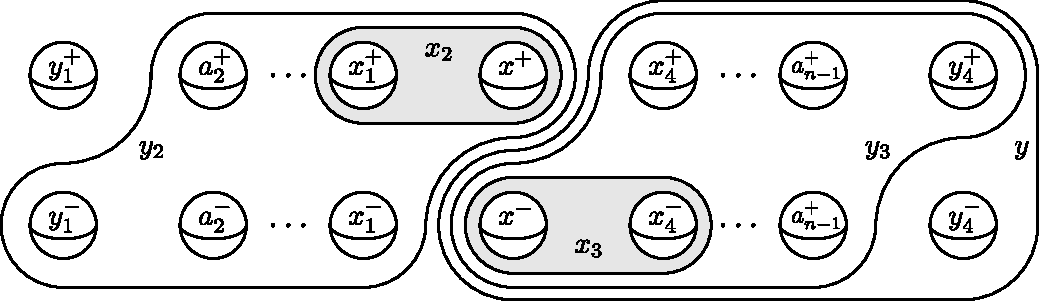
\includegraphics[width=\textwidth]{spheresagain.pdf}
\caption{
The manifold $M_n|\{a_i\}_{i=1}^n$ is $S^3$ with $2n$ balls removed.
We obtain $M_n$ by again identifying the spheres with $+$ and $-$ labels via a vertical reflection.
The spheres $\Sigma'=\{x_i,y_i\}_{i=1}^4$ are such that $M_n|\Sigma'$ contains $x$ and $y$ in disjoint copies of $M_{0,4}$. The $M_{0,4}$ containing $x$ (identify $x^+$ and $x^-$) is shaded. The $M_{0,4}$ containing $y$ is the exterior of $y_2$ and $y_3$.
}
\label{fig:spherediagram}
\end{figure}

\medskip \noindent \emph{Case 2.} Suppose $\Sigma=\{x,y\}$ has $m=2$ spheres.
Choose a collection $\Sigma'$ of disjoint nonseparating spheres such that  there are two separate components of $M_n|\Sigma'$ homeomorphic to $M_{0,4}$ and containing $x$ and $y$ respectively.
We can construct $\Sigma'$ as follows.
$M_n|\Sigma$ has two components, homeomorphic to $M_{k,2}$ and $M_{n-k-1,2}$.
So we have a set of spheres $\{a_i\}_{i=1}^n$ coconnected in $M_n$ disjoint from $y$ with $a_{k+1}=x$.
Choose $x_2,x_3,y_2,y_3$ as shown in figure \ref{fig:spherediagram} and relabel $a_1=y_1$, $x_{1}=a_k$, $x_4=a_{k+2}$, $y_4=a_n$. 
Then 
$\{x_1,\ldots, x_4\}$ (resp. $\{y_1, \ldots, y_4\}$ are the boundary spheres of a component of $M|\Sigma'$ homeomorphic to $M_{0,4}$ and containing $x$ (resp. $y$).
Further $\{x,x_1,x_2\}$ and $\{x,x_3,x_4\}$ are genus 0 bounding triples. Let $\Sigma' =\{x_i,y_i\}_{i=1}^4$.



By Case 1 we have that $\{\phi(x_1), \ldots, \phi(x_4)\}$ is a genus 0 bounding $4$-tuple and $\{\phi(x),\phi(x_1),\phi(x_2)\}$ and $\{\phi(x),\phi(x_3),\phi(x_4)\}$ are genus 0 bounding triples. 
So $\{\phi(x_1), \ldots, \phi(x_4)\}$ define a component of $M|\Sigma'$ homeomorphic to $M_{0,4}$ and containing $\phi(x)$.

If $\{x_1, \ldots, x_4\} \neq \{y_1, \ldots, y_4\}$ then 
 $\phi(x)$ and $\phi(y)$ lie in disjoint $M_{0,4}$ homeomorphic components of $M|\phi(\Sigma')$.
Then  $\phi(x)$ and $\phi(y)$ are are disjoint. They are also not adjacent in $\coc n$, so they are bounding a pair.

Suppose $\{x_1, \ldots, x_4\} = \{y_1, \ldots, y_4\}$.
Then $n=3$ and $M_3|\{x_i\}_{i=1}^4$ is homeomorphic to two copies of $M_{0,4}$.
As $x,y$ form a bounding pair, the bounding triples must be
$\{x,x_1,x_2\}$, $\{x,x_3,x_4\}$, $\{y,x_1,x_2\}$, and $\{y,x_3,x_4\}$.
Then the $\phi$ image of these triples are
bounding triples giving $\phi(x)$ and $\phi(y)$ contained in disjoint $M_{0,4}$.
Then $\phi(x)$ and $\phi(y)$ are disjoint and must form a bounding pair.
\end{proof}


\bibliography{spherecomplex}{}
\bibliographystyle{plain}
\end{document}
